\documentclass[titlepage,a4paper]{article}

\usepackage{a4wide}
\usepackage[colorlinks=true,linkcolor=black,urlcolor=blue,bookmarksopen=true]{hyperref}
\usepackage{bookmark}
\usepackage{fancyhdr}
\usepackage[spanish]{babel}
\usepackage[utf8]{inputenc}
\usepackage[T1]{fontenc}
\usepackage{graphicx}
\usepackage{float}

\pagestyle{fancy} % Encabezado y pie de página
\fancyhf{}
\fancyhead[L]{TP1 - L. De Angelis Riva}
\fancyhead[R]{Algoritmos y Programación III - FIUBA}
\renewcommand{\headrulewidth}{0.4pt}
\fancyfoot[C]{\thepage}
\renewcommand{\footrulewidth}{0.4pt}

\begin{document}
\begin{titlepage} % Carátula
	\hfill
\includegraphics[width=6cm]{LogoFiuba3.0HD.png}
    \centering
    \vfill
    \Huge \textbf{Trabajo Práctico 1 — Smalltalk}
    \vskip2cm
    \Large [7507/9502] Algoritmos y Programación III\\
    Curso 2 \\ % Curso 1 para el de la tarde y 2 para el de la noche
    Primer cuatrimestre de 2020 
    \vfill
    \begin{tabular}{ | l | l | } % Datos del alumno
      \hline
      Alumno: & De Angelis Riva, Lukas Nahuel \\ \hline
      Número de padrón: & 103784 \\ \hline
      Email: & ldeangelis@fi.uba.ar \\ \hline
  	\end{tabular}
    \vfill
    \vfill
\end{titlepage}

\tableofcontents % Índice general
\newpage

\section{Introducción}\label{sec:intro}
El presente informe reúne la documentación de la solución del primer trabajo práctico de la materia Algoritmos y Programación III que consiste en desarrollar una aplicación de un sistema de cálculo del presupuesto más baratos para pintar una cantidad de metros cuadrados. El lenguaje de programación utilizado es Smalltak y fue desarrollado en Pharo, utilizando los conceptos del paradigma de la orientación a objetos vistos hasta ahora en el curso.

\section{Supuestos}\label{sec:supuestos}
% Deberá contener explicaciones de cada uno de los supuestos que el alumno haya tenido que adoptar a partir de situaciones que no estén contempladas en la especificación.

Consideraciones no explicitadas en la lógica del programa:
\begin{itemize}
    \item Es válido que el usuario registre dos pintores con las mismas características\\
    En dicho caso la colección de pintores tendrá dos pintores que se comportarán idénticamente.
    \item Es válido que el usuario registre un mismo pintor (mismo nombre) con distintas técnicas y/o con diferente valor por hora.
    \item El presupuesto siempre será el mínimo, pero en caso de que haya múltiples presupuestos con mismo valor, se devolverá el que corresponda al pintor que antes fue registrado.
    \item No se podrá registrar un pintor con nombre vacío ni crear una pintura sin nombre.
\end{itemize}
\section{Modelo de dominio}\label{sec:modelo}
% Explicación concisa del diseño general del trabajo.

El trabajo práctico consiste en la interacción entre las clases que forman parte de la lista que se muestra más adelante.
Básicamente se encarga de barajar distintos presupuestos para pintar una cantidad de metros cuadrados, respecto a una colección de Pintores y una determinada Pintura, siendo el objetivo calcular el mínimo presupuesto. Existen dos tipos de técnica de pintura, estas son: \textit{técnica de pincel y técnica de rodillo} cada una teniendo sus singularidades abajo determinadas.
 Las clases que participan en el programa son:
\begin{itemize}
    \item \textbf{AlgoFix:} En esencia es la API. El usuario se comunicará con la clase y esta le proveerá los datos solicitados en base a los datos ingresados.
    \item \textbf{PintorPincel:} Modela la estructura de un pintor con la herramienta pincel.
    Tendrá las consideraciones apropiadas para su técnica de pintura, estas son:
    \iten\begin{itemize}
        \item Horas para pintar un metro cuadrado: 2.
        \item Litros para pintar un metro cuadrado: 4.
        \item Aplicará un descuento del 50\% si los metros cuadrados a pintar superan los 40 metros cuadrados.
    \end{itemize}
    \item \textbf{PintorRodillo:} Modela la estructura de un pintor con la herramienta rodillo.
    Tendrá las consideraciones apropiadas para su técnica de pintura, éstas son:
    \item\begin{itemize}
        \item Horas para pintar un metro cuadrado: 1.
        \item Litros para pintar un metro cuadrado: 5.
    \end{itemize}
    \item \textbf{Pintura:} Modela la estructura pintura, es la encargada de guardar la información que tiene una pintura y además la clase encargada de comunicar a la clase Pintor con la clase Presupuesto seleccionando los datos necesarios para el cálculo del mismo.
    \item \textbf{Presupuesto:} Es la estructura que se encarga de interpretar los datos y con ellos calcular el presupuesto final.

\end{itemize}

\section{Diagramas de clase}\label{sec:diagramasdeclase}
% Uno o varios diagramas de clases mostrando las relaciones estáticas entre las clases.  Puede agregarse todo el texto necesario para aclarar y explicar su diseño. Recuerden que la idea de todo el documento es que quede documentado y entendible cómo está implementada la solución.
\begin{figure}[H]
\centering
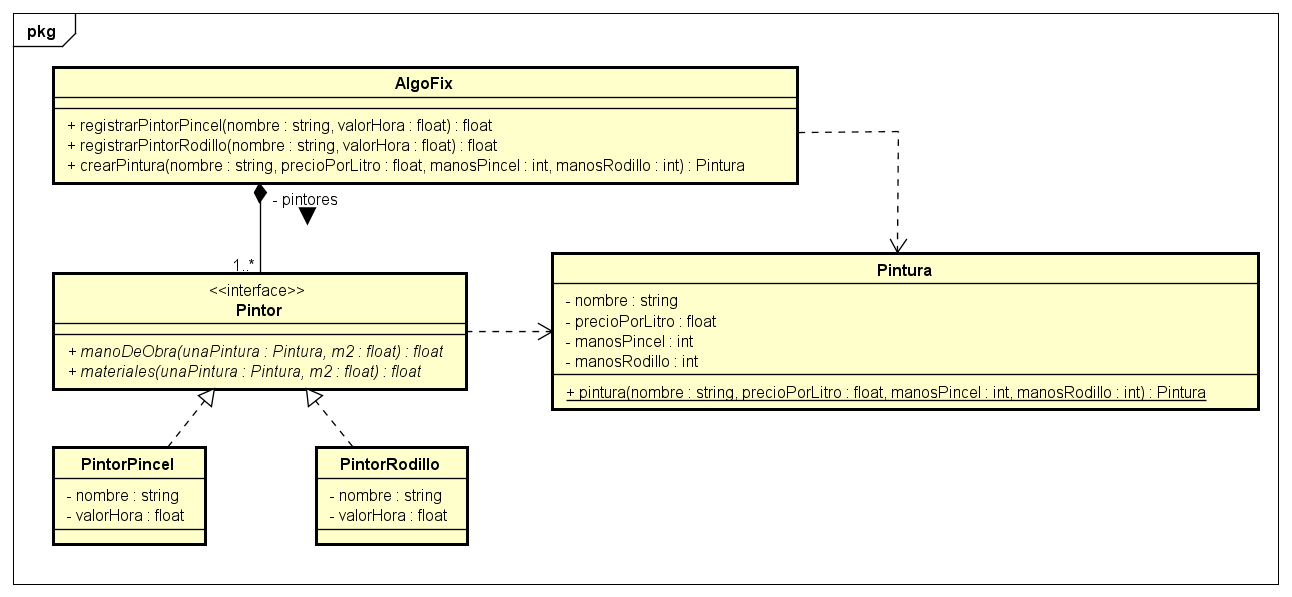
\includegraphics[width=1\textwidth]{crearAPP.png}
\caption{\label{fig:class01}Organización de las clases.}
\end{figure}
La figura 1 muestra como se relacionan las clases en la fase de \textit{arrange}.\\\\
AlgoFix almacenará una colección de Pintores.\\
Las clases PintorPincel y PintorRodillo implementan la interfaz \textit{Pintor}.\\
AlgoFix utiliza una Pintura cuando requiere crear una pintura.\\
El pintor utiliza una Pintura cuando requiere calcular la mano de obra y los materiales.

\begin{figure}[H]
\centering
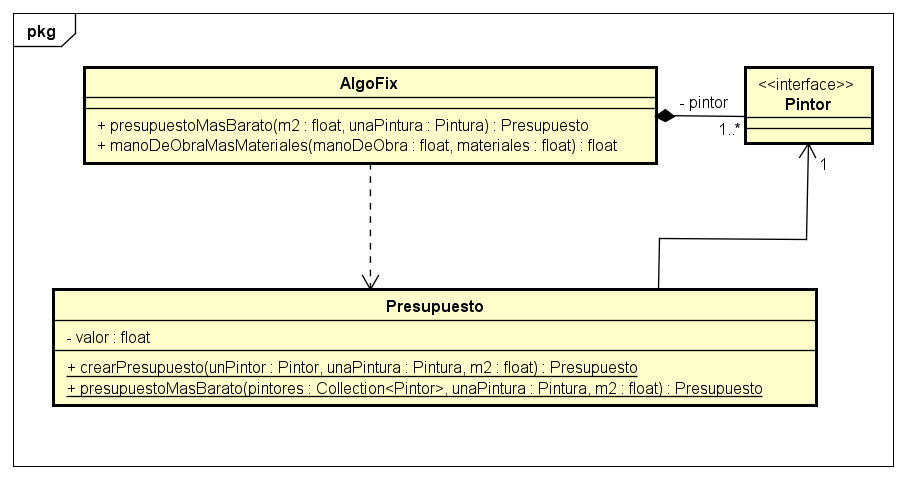
\includegraphics[width=1\textwidth]{AlgoPresupuesto.png}
\caption{\label{fig:class01} .}
\end{figure}
La figura 2 muestra como se relaciona AlgoFix con la clase presupuesto.

\begin{figure}[H]
\centering
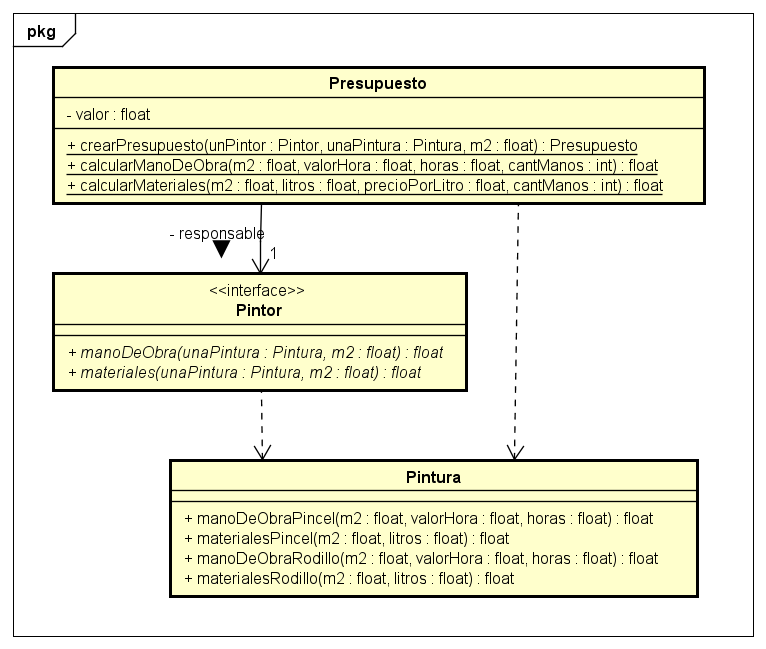
\includegraphics[width=1\textwidth]{PPP.png}
\caption{\label{fig:class01} .}
\end{figure}
La figura 3 muestra como se relaciona la clase Presupuesto con las clases Pintor y Pintura.
\section{Detalles de implementación}\label{sec:implementacion}
% Explicaciones sobre la implementación interna de algunas clases que consideren que puedan llegar a resultar interesantes.

\subsection{AlgoFix}
La clase AlgoFix guarda una colección de Pintores, para ello utilicé una OrderedColection.\\
Los Pintores se agregaran a la colección mandando el mensaje registrarPintorDePincel/ registrarPintorDeRodillo de la clase AlgoFix como lo muestra la figura 1.\\
Para esto se instanciará un Pintor de la clase correspondiente y se agregará a la colección\\
Ejemplo:
\begin{verbatim}
registrarPintorDeRodillo: unNombre conValorHora: unValorHora\end{verbatim}\\\begin{verbatim}
	pintores add:( PintorRodillo deNombre: unNombre conValorHora: unValorHora)
\end{verbatim}
Analogamente para registrar a un Pintor de rodillo.\\

Para conseguir el mínimo Presupuesto para pintar los metros cuadrados AlgoFix le delega la responsabilidad a Presupuesto, brindándole la colección de pintores.\\
Implementación:
\begin{verbatim}
presupuestoMasBaratoParaPintarMetrosCuadrados: metrosCuadrados
  conPintura: unaPintura\end{verbatim}\\  \begin{verbatim}
        ^(Presupuesto presupuestoMasBarato: pintores
          conPintura: unaPintura
          conMetrosCuadrados: metrosCuadrados)

\end{verbatim}

\subsection{Presupuesto}
La clase Presupuesto tiene la responsabilidad de hacer la cuenta del cálculo del valor del presupuesto, por lo que, cuando se llama al constructor se le pasa el Pintor, la Pintura y la cantidad de metrosCuadrados.
\begin{verbatim}
conResponsable: unPintor conPintura: unaPintura conMetrosCuadrados:
metrosCuadrados
    	|presupuesto|
    	presupuesto := self new.
    	presupuesto asignarResponsable: unPintor.
    	presupuesto asignarValorCon: unPintor conPintura: unaPintura
    	    conMetrosCuadrados: metrosCuadrados.
    	^presupuesto.
\end{verbatim}
El mensaje de instancia asignarValor asignará a la variable de instancia el valor del presupuesto.
\begin{verbatim}
asignarValorCon: unPintor conPintura: unaPintura
  conMetrosCuadrados: metrosCuadrados

        valor := (self class)
        manoDeObra: (self manoDeObraConResponsable: unPintor 
          conPintura: unaPintura
          conMetrosCuadrados: metrosCuadrados) 
        masMateriales: (self materialesConResponsable: unPintor
          conPintura: unaPintura
          conMetrosCuadrados: metrosCuadrados).
\end{verbatim}
\subsection{Pintor}
    La diferencia entre un Pintor de pincel y un pintor de rodillo es el mensaje que le manda a la pintura.\\
    \\Ejemplo al calcular los materiales:
    \begin{itemize}
    \item PintorPincel
    \begin{verbatim}
calcularMaterialesConPintura: unaPintura
  conMetrosCuadrados: metrosCuadrados.

    (metrosCuadrados < 0) ifTrue:[MetrosCuadradosNegativos signal].
    
    ^(unaPintura calcularMaterialesDePincelConMetrosCuadrados:
        metrosCuadrados
        conLitros: litrosPincel).
    \end{verbatim}
    
    \item{PintorRodillo}
    \begin{verbatim}
    calcularMaterialesConPintura: unaPintura
      conMetrosCuadrados: metrosCuadrados.
	    
	    (metrosCuadrados < 0) ifTrue:[MetrosCuadradosNegativos signal].
	    
	    ^(unaPintura calcularMaterialesDeRodilloConMetrosCuadrados:
	        metrosCuadrados
	        conLitros: litrosRodillo).
    \end{verbatim}
\end{itemize}
Algo similar ocurre al calcular la mano de obra.\\\\
Es debido a esto que he decidido utilizar una interfaz en vez de una herencia, ya que PintorPincel y PintorRodillo tienen un comportamiento muy distinto en el sentido de que le mandan diferentes mensajes a la Pintura. Por lo que ambas clases deberían redefinir los (únicos) métodos que poseen.\\
Además de que el PintorPincel implementa un descuento y el PintorRodillo no.\\
Como se ve en la implementación, el Pintor delega la responsabilidad de calcular el precio de los materiales / manoDeObra en la instancia de Pintura.

\subsection{Pintura}
    La instancia Pintura tendrá los 4 mensajes mostrados en la figura 3.\\
    Y tendrá dos mensajes de clase para modularizar código.\\
    Ejemplo para calcular los materiales con la técnica pintura\\\\
    Mensaje de instancia:
    \begin{verbatim}
    calcularMaterialesDePincelConMetrosCuadrados: metrosCuadrados
      conLitros: litros
    
	        ^((self class) calcularMaterialesConMetrosCuadrados: metrosCuadrados 
	            conLitros: litros
	            conPrecioPorLitros: precioPorLitro 
	            conCantManos: manosPincel).
    \end{verbatim}
    Mensaje de clase:
    \begin{verbatim}
    
    calcularMaterialesConMetrosCuadrados: metrosCuadrados conLitros: litros
    conPrecioPorLitros: precioPorLitro conCantManos: cantManos


            ^(Presupuesto calcularMaterialesConMetrosCuadrados: metrosCuadrados
    	        conLitros: litros
    	        conPrecioPorLitro: precioPorLitro
    	        conManoHerramienta: cantManos).
    \end{verbatim}
    La única diferencia al calcular materiales con rodillo es que varía en la cantidad de manos de la técnica requerida, por lo que he decidio modularizar el comportamiento en dicho mensaje de clase.
    
\section{Excepciones}\label{sec:excepciones}
% Explicación de cada una de las excepciones creadas y con qué fin fueron creadas.

\begin{description}

\item[CantidadHorasNegativo] Se levantará esta excepción cuando se envíe una cantidad de horas negativa para calcular la mano de obra.

\item[LitrosNegativos] Se levantará esta excepción cuando se envíe una cantidad de litros negativos para calcular materiales.

\item[ManoDeObraNegativa] Se levantará esta excepción cuando se envíe el valor de la mano de obra negativo cuando se pida sumarlo junto a los materiales.

\item[MaterialesNegativos] Se levantará esta excepción cuando se envíe el valor de los materiales negativo cuando se pida sumarlo junto a la mano de obra.

\item[ManosPincelInvalido] Se levantará esta excepción en caso de que se intente instanciar una pintura con manos cantidad de manos pincel negativas.

\item[ManosRodilloInvalido] Se levantará esta excepción en caso de que se intente instanciar una pintura con manos cantidad de manos rodillo negativas.


\item[MetrosCuadradosNegativos] Se levantará esta excepción cuando se envíe a calcular el presupuesto de metroscuadrados negativos.

\item[NoHayPintores] Se levantará esta excepción cuando se intente acceder a una colección de pintores vacía.

\item[NoHayPresupuestos] Se levantará esta excepción cuando se intente obtener el presupuesto más barato de una colección de presupuestos vacía.

\item[NombreInvalido] Se levantará esta excepción cuando se intente instanciar un objeto con nombre vacío.

\item[PrecioPorLitroNegativo] Se levantará esta excepción cuando se intente instanciar una pintura con precio por litro negativo, o cuando se intente crear un presupuesto con precio por litros negativos.

\item[ValorHoraNegativo] Se levantará esta excepción cuando se intente instanciar un pintor con valor por hora negativo, o cuando se intente crear un presupuesto con valor por hora negativo.


\end{description}

\section{Diagramas de secuencia}\label{sec:diagramasdesecuencia}
% Mostrar las secuencias interesantes que hayan implementado. Pueden agregar texto para explicar si algo no queda claro.

Los siguientes diagramas de secuencia muestran cómo será la ejecución del siguiente programa:
\begin{verbatim}
	|algoFix venier presupuesto_15m2 presupuesto_50m2|
	
	algoFix := AlgoFix new.
	
	algoFix registrarPintorDePincel: 'Diego'
	  conValorHora: 500.
	  
	algoFix registrarPintorDeRodillo: 'Tomás'
	  conValorHora: 500.
	
	algoFix registrarPintorDePincel: 'Pablo'
	  conValorHora: 600.
	
	venier := algoFix crearPintura: 'Venier'
	  conPrecioPorLitro: 150
	  manosPincel: 2
	  manosRodillo: 1.
	
	presupuesto_15m2 := algoFix presupuestoMasBaratoParaPintarMetrosCuadrados: 15
	  conPintura: venier.
    
	presupuesto_50m2 := algoFix presupuestoMasBaratoParaPintarMetrosCuadrados: 50
	    conPintura: venier.
    
\end{verbatim}

\begin{figure}[H]
\centering
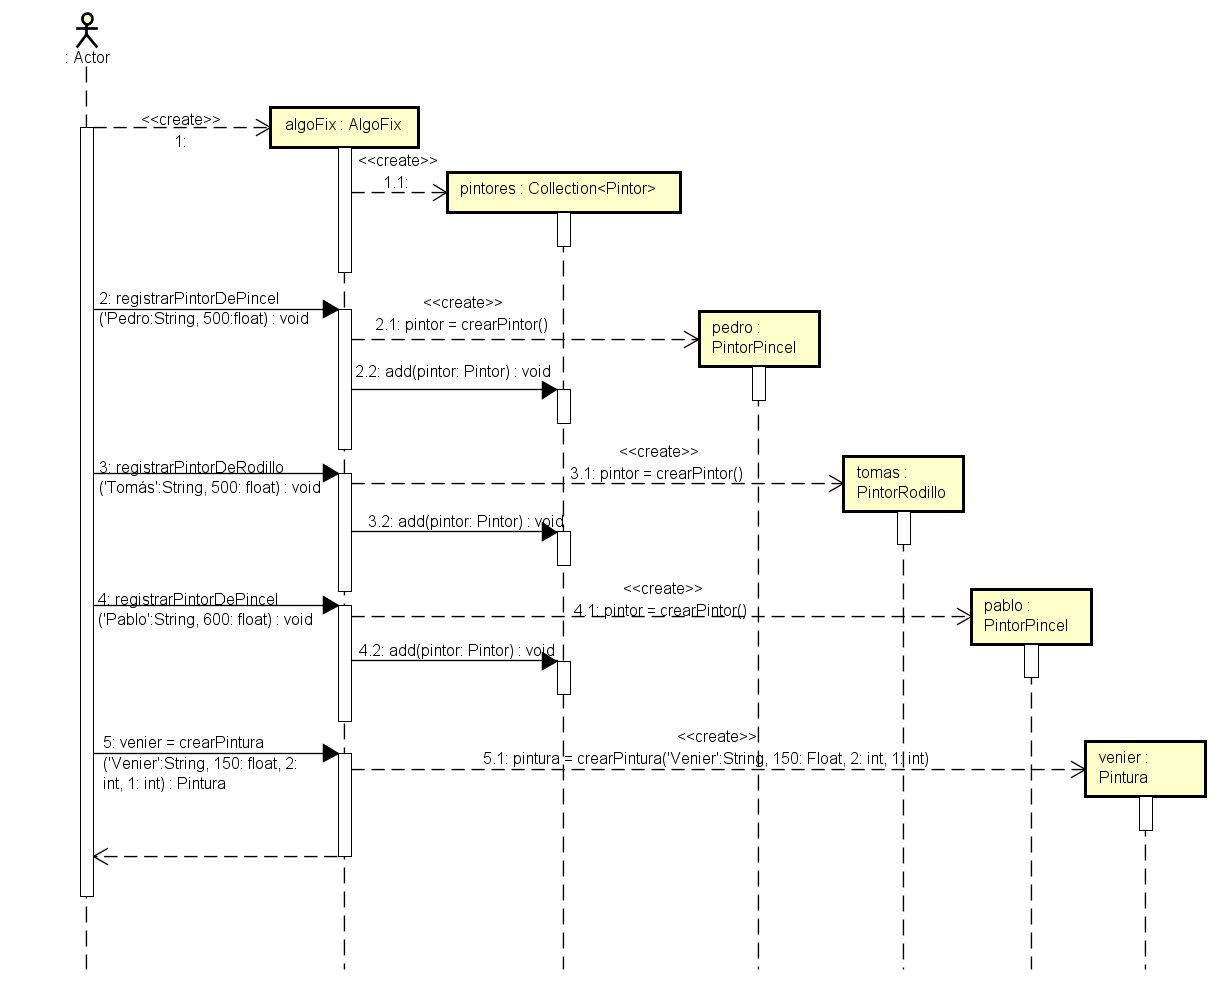
\includegraphics[width=1\textwidth]{Secuencia1Arrange.png}
\caption{\label{fig:seq01} Fase del arrange}
\end{figure}

La figura 4 muestra cómo se comunica algoFix con las demás clases del programa en la fase de arrange.\\
Crea pintores y los añade a una colección; Además crea las pinturas y las devuelve.


\begin{figure}[H]
\centering
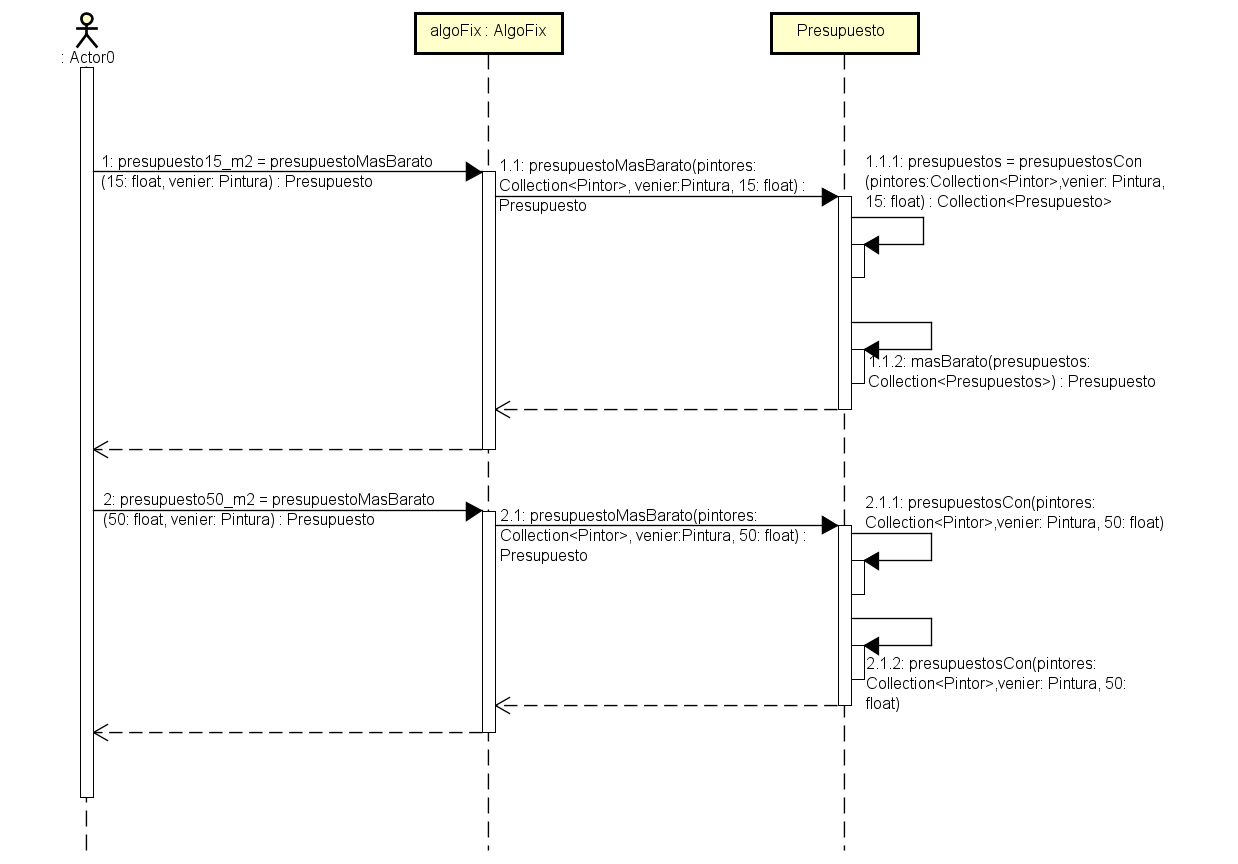
\includegraphics[width=1.1\textwidth]{Secuencia2ACT.png}
\caption{\label{fig:seq02} Fase de act}
\end{figure}

El mensaje \textit{presupuestoMasBarato} se envía a la clase Presupuesto; lo que se ejecutará en este método se verá detallado en las figuras 6, 7 y 8.\\

Se puede ver detalladamente que el comportamiento de AlgoFix depende explícitamente de las otras clases que participan. De hecho, delega todo su comportamiento en las clases que utiliza,
pues su única labor es organizar y comunicar a las demás clases. 


\begin{figure}[H]
\centering
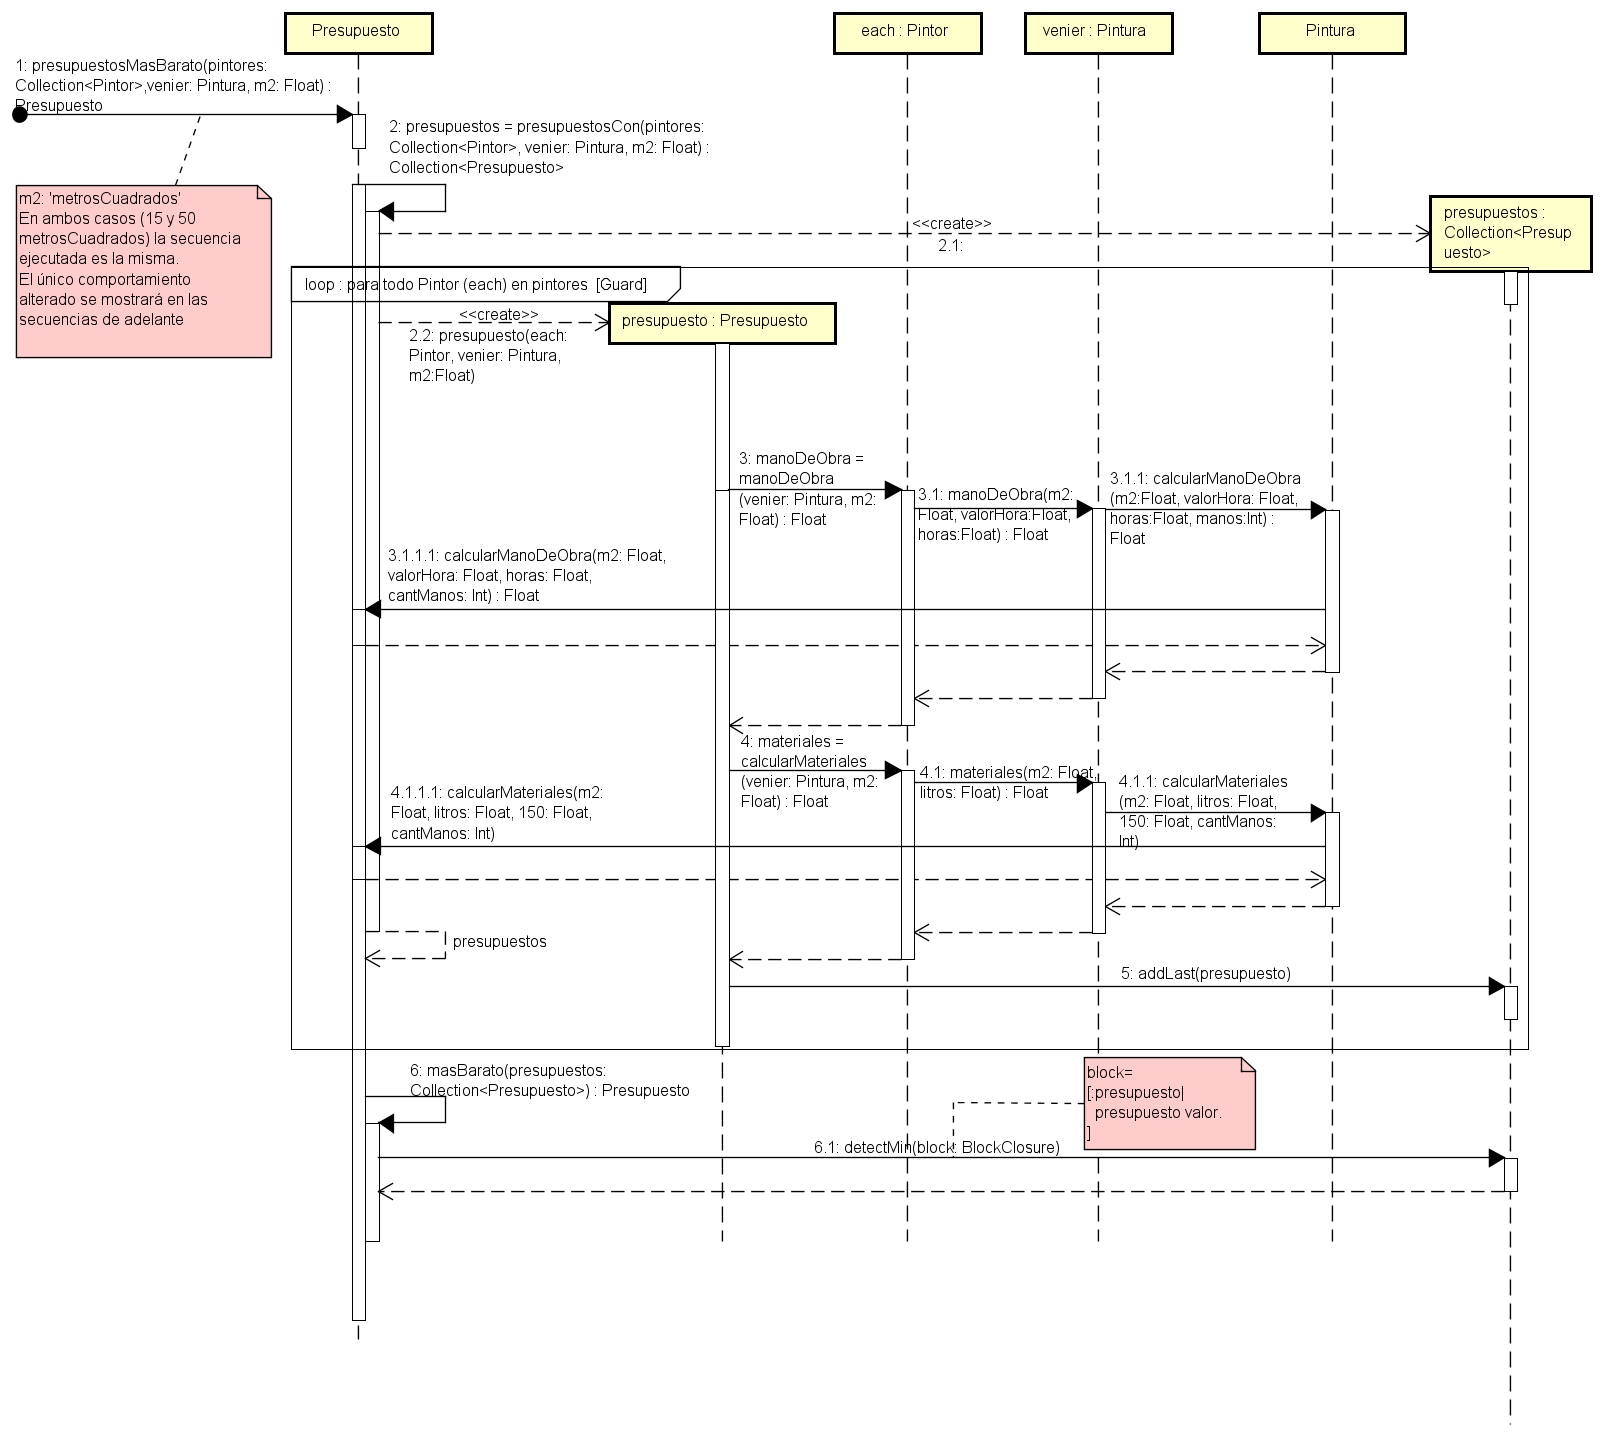
\includegraphics[width=1.1\textwidth]{Secuencia3CalcularPresupuestoGRAL.png}
\caption{\label{fig:seq02} Cálculo del mínimo presupuesto}
\end{figure}

Este diagrama de secuencia muestra qué sucede cuando se manda el mensaje de calcular el presupuesto más barato con una colección de pintores creada a partir del programa simulado, justo como se muestra en la figura 4.
\\Se abstrae la idea de Pintor en la colección, y también la comunicación que tienen con el objeto venier haciendo uso del polimorfismo, en las figuras 7, 8 y 9 se mostrará qué mensajes se mandarán en cada caso de los pintores posibles.
\\Como se muestra en la figura, se crean instancias de presupuesto y se añaden a la colección de presupuestos para que más adelante se busque el mínimo presupuesto utilizando el mensaje detectMin de las colecciones.


\begin{figure}[H]
\centering
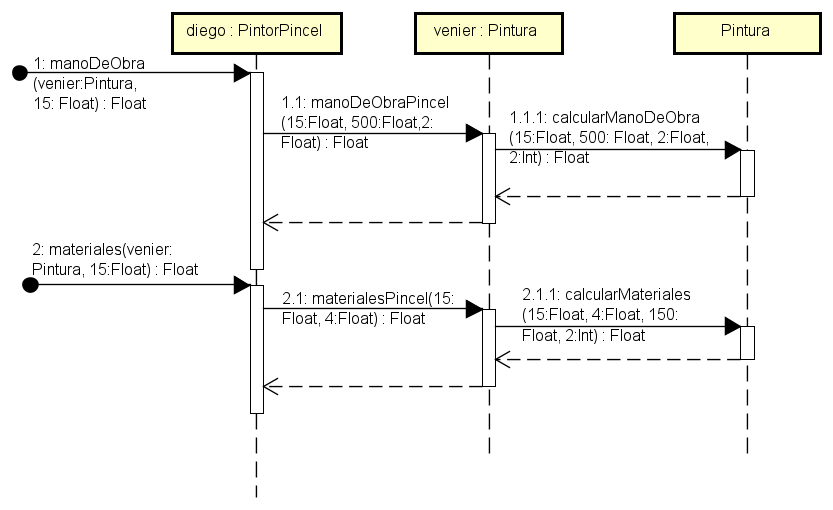
\includegraphics[width=1.1\textwidth]{Secuencia4_1PincelSinDescuento.png}
\caption{\label{fig:seq02} Secuencia para PintorPincel sin descuento}
\end{figure}
Como se puede observar en la figura 6, un Pintor de Pincel llamará a los métodos de Pintura que refieran a la técnica de pincel.
Por lo que, cuando un pintor de la colección que sea instancia de la clase PintorPincel procederá a realizar el procedimiento de la figura 6.

\begin{figure}[H]
\centering
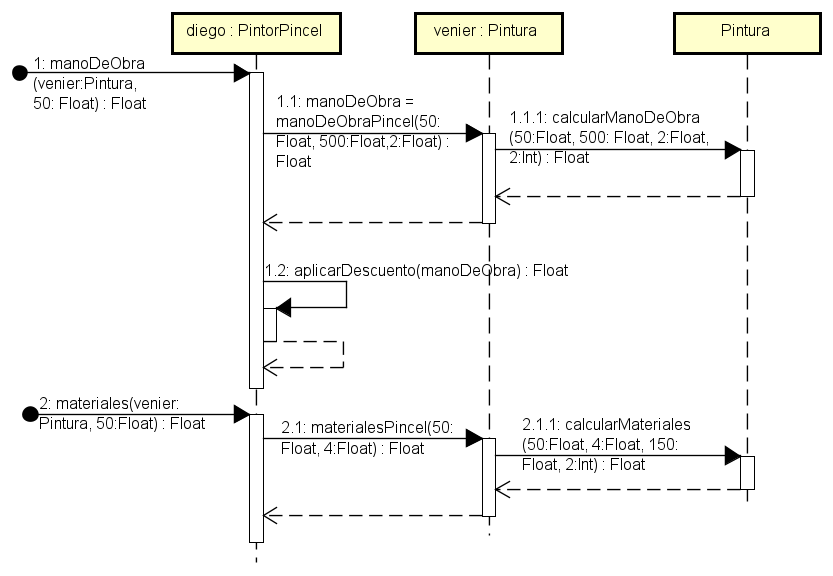
\includegraphics[width=1.1\textwidth]{Secuencia4_2PincelDescuento.png}
\caption{\label{fig:seq02} Secuencia para PintorPincel con descuento}
\end{figure}
A diferencia de la figura 7, dado que el pintor de pincel recibió una cantidad de 50 metros cuadrados a pintar superior a 40 metros cuadrados, se aplicará un descuento.
\begin{figure}[H]
\centering
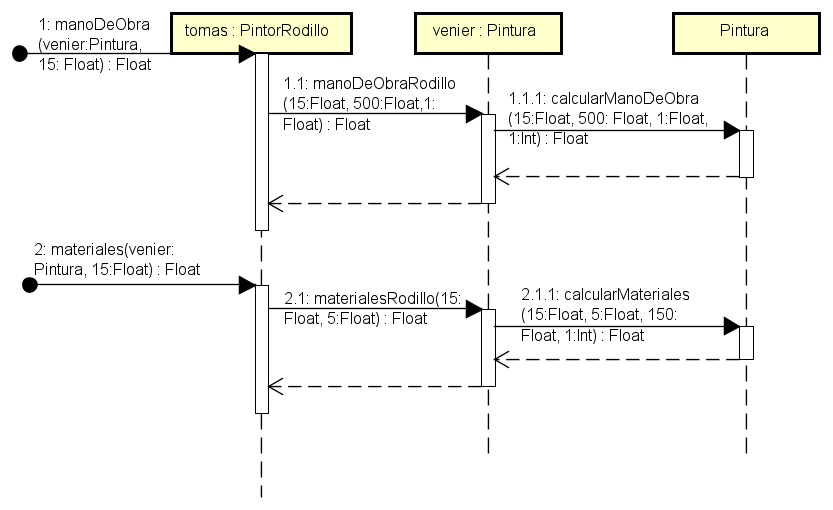
\includegraphics[width=1.1\textwidth]{Secuencia5_PincelRodillo.png}
\caption{\label{fig:seq02} Secuencia para PintorRodillo}
\end{figure}
Como se puede observar en la figura 9, un Pintor de Rodillo llamará a los métodos de Pintura que refieran a la técnica de rodillo.
Por lo que, cuando un pintor de la colección que sea instancia de la clase PintorRodillo procederá a realizar este procedimiento.
Dado que el pintor de rodillo no aplica descuento en ninguna circunstancia la figura 9 representa idénticamente el comportamiento del pintor de rodillo en caso de que reciba los 50 metros cuadrados a pintar.



\end{document}
